
\chapter{Операциони појачавач и индуктивни елементи}

\section{Напонски диференцијални појачавач}
Поједностављен модел реалног 
напонског 
диференцијалног појачавача без меморије, приказан на слици \ref{fig:da1}, карактерисан је својом улазном отпорношћу $R_{\rm u}$, 
излазном отпорношћу $R_{\rm i}$ и напонским појачањем $A$ напонски
контролисаног напонског генератора.  
%
\begin{figure}[ht!]
\centering
    \begin{subfigure}[c]{0.32\textwidth}
    \centering
        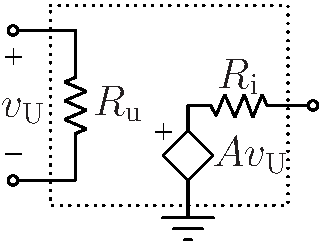
\includegraphics[scale=0.8]
        {fig/diff-amp.pdf}
        \caption{Унутрашња структура.}
        \label{fig:da1}
    \end{subfigure}
    %
    \begin{subfigure}[c]{0.32\textwidth}
    \centering
        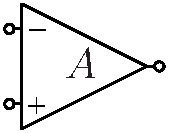
\includegraphics[scale=0.8]
        {fig/diff-amp-symb.pdf}
        \caption{Симбол.}
        \label{fig:da2}
    \end{subfigure}
\caption{Уз диференцијални појачавач}
\end{figure}
Има два улаза, један инвертујући 
(обележен са „-“) и један неинвертујући (обележен са „+“). Шематски симбол представљен је на 
слици \ref{fig:da2}.
Добар диференцијални напонски појачавач задовољава да су $R_{\rm u}\to\infty$, 
$R_{\rm i}\to0$. Такав диференцијални појачавач практично 
представља идеалан напоном контролисан напонски генератор, када је 
$v_{\rm I} = A v_{\rm U}$.

\section{Негативна повратна спрега}
\begin{figure}[b!]
    \centering
    \begin{subfigure}[c]{0.32\textwidth}
    \centering
        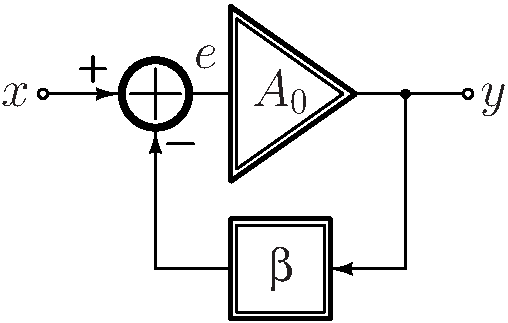
\includegraphics[scale=0.5]
        {fig/black-model.pdf}
        \caption{Блеков модел.}
        \label{fig:black}
    \end{subfigure}
    ~ %add desired spacing between images, e. g. ~, \quad, \qquad, \hfill etc. 
      %(or a blank line to force the subfigure onto a new line)
    \begin{subfigure}[c]{0.32\textwidth}
    \centering
        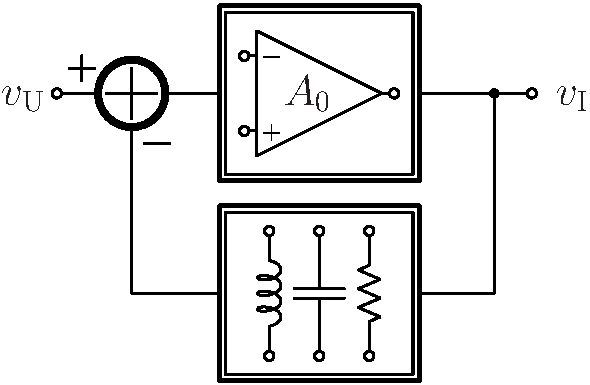
\includegraphics[scale=0.5]
        {fig/black-model-op.pdf}
        \caption{Блеков модел, са ОП.}
        \label{fig:op2}
    \end{subfigure}
    ~ %add desired spacing between images, e. g. ~, \quad, \qquad, \hfill etc. 
    %(or a blank line to force the subfigure onto a new line)
    \begin{subfigure}[c]{0.32\textwidth}
    \centering
        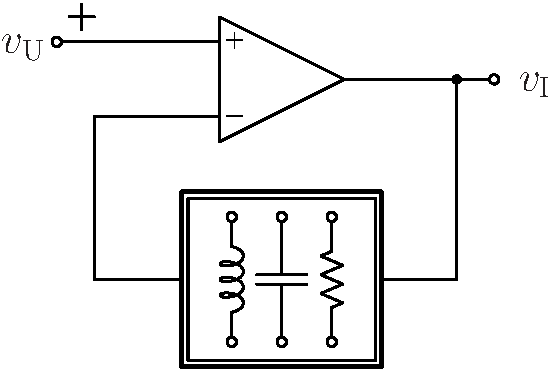
\includegraphics[scale=0.5]
        {fig/black-model-op-conc.pdf}
        \caption{Операциони појачавач, пример.}
        \label{fig:black3}
    \end{subfigure}
    \caption{Уз увођење принципа операционог појачавача.}
\end{figure}
%
Концепт који суштински мења начин употребе диференцијалног појачавача 
је са принцип реакције (повратне спреге). Блеков модел система са реакцијом 
приказан је 
блок дијаграмом
на слици \ref{fig:black}. У овом моделу, главни 
појачавач има појачање $A_0$ а мрежа повратне спреге појачање 
$\upbeta$. Појачање целокупног система се добија на основу 
блок дијаграма:
\begin{eqnarray}
	&e = x - \upbeta y \\
	&y = A_0 e, 
\end{eqnarray}
одакле се сређивањем добија појачање целог система
$A = \dfrac{y}{x} = \dfrac{A_0}{1 + \upbeta A_0}$.   
%
Сигнал $e$ назива се још и \textit{сигналом грешке}, а може се 
изразити преко улазног сигнала као $e = \dfrac{1}{1 + \upbeta A_0}x$.
Повратна спрега посебно добија на вредности када се размотри 
главни појачавач са веома великим појачањем, $A_{0} \to \infty$. У том случају су $A_{\infty} = \lim_{A_{0} \to \infty} 
\dfrac{A_0}{1 + \upbeta A_0} = \dfrac{1}{\upbeta}$ и 
$e_{\infty} = \lim_{A_{0} \to \infty} 
\dfrac{1}{1 + \upbeta A_0} = 0$. Односно, за довољно велико појачање 
главног појачавача, \myul{карактеристике система са 
повратном спрегом диктира мрежа повратне спреге}. Посебно, ова топологија се 
може реализовати, на пример, помоћу операционог појачавача 
са пасивном мрежом повратне спреге, што је илустровано на слици 
\ref{fig:op2}. Према пређашњој дискусији, карактеристике оваквог 
система зависиће само од мреже повратне спреге ако је напонско 
појачање оваквог доброг диференцијалног појачавача веома велико. 
Такав диференцијални појачавач, 
ког кога је још и $A_0 \to \infty$, назива се \textbf{идеални 
операциони појачавач}. Идеални операциони појачавач најчешће 
обележавамо изостављањем ознаке 
напонског
појачања. Разлика улазног и повратног сигнала која се 
појачава, у ваљано одабраној топологији
(нпр. слика \ref{fig:black3}), 
мора бити разлика напона на улазима операционог појачавача, на основу чега
резултат да је $e_{\infty} \to 0$ повлачи 
то да се у оваквом режиму \myul{изједначавају напони инвертујућег
и неинвертујућег улаза}. Важно је нагласити, да ово није једина 
тополошка опција, већ да се улазни и излазни сигнал могу 
одузимати и на другачије начине, што се може видети на разним 
примерима (нпр. инвертујући појачавач). 
%
%

%
Коначно, уколико је операциони појачавач примењен у режиму 
повратне спреге онда се он може анализирати помоћу три правила која следе из пређашње анализе: \\

\shadowbox{
\begin{minipage}{0.5\textwidth}
\textbf{\myul{Идеалан операциони појачавач}}
\begin{itemize}
\item $i_+ = i_- = 0$ (јер је $R_{\rm u} \to 0$)
\item $v_+ = v_-$ (јер је $e_{\infty} \to 0$)
\item Излаз има произвољну вредност, тако да су 
задовољени пређашњи услови, $-\infty < v_{\rm OP} < \infty$.
\end{itemize}
\end{minipage}
%
\begin{minipage}{0.4\textwidth}
\begin{flushright}
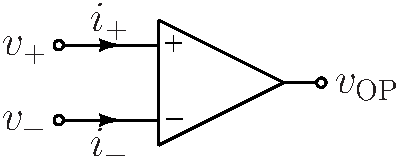
\includegraphics[scale=0.8]{fig/op.pdf}
\end{flushright}
\end{minipage}
}

\section{Индуктивни трансформатори}
\subsection{Спрегнути калемови}
Физички модел на коме су утемељени индуктивни трансформатори је модел 
спрегнутих калемова. Магнетска спрега два посматрана линеарна намотаја,
индуктивности $L_1$ и $L_2$ описује се
међусобном индуктивношћу $L_{\rm 12} = L_{\rm 21}$ (за реципрочне средине). Коефицијент магнетске спреге се дефинише као апсолутна 
вредност међусобне индуктивности сведена на јединицу геометријске
средине индуктивности појединих намотаја: 
$k = \dfrac{|L_{12}|}{\sqrt{L_1 L_2}}$, за знак међусобне 
индуктивности је одређен и смером мотања намотаја и шематски 
се обележава тачкама. Без додатних услова овакав пар спрегнутих 
калема описан је једначинама у временском домену:

\begin{center}
\shadowbox{
\begin{minipage}{0.3\textwidth}
\textbf{\myul{Пар спрегнутих калемова}}
\vspace*{0.5em}
\begin{itemize}
\item $v_1 = L_1 \dfrac{\de i_1}{\de t} + 
L_{12} \dfrac{\de i_2}{\de t}$ 
\item $v_2 = L_{12} \dfrac{\de i_1}{\de t} + 
L_{2} \dfrac{\de i_2}{\de t}$ 
\end{itemize}
\end{minipage}
%
\begin{minipage}{0.2\textwidth}
\begin{flushright}
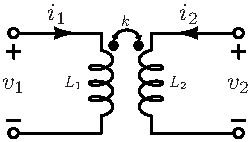
\includegraphics[scale=0.8]{fig/spregnuti.pdf}
\end{flushright}
\end{minipage}
}
\end{center}

За решавање проблема са спрегнутим калемовима, уколико су калемови 
кратко спојени са једне стране неретко је веома згодно прво обавити \textit{распрезање калемова} трансфигурацијом у еквивалентну
Т--мрежу као на слици \ref{raspreg}. Будући да је ово трансфигурација, 
то подразумева да су ове две мреже еквивалентне у сваком смислу.

\begin{figure}[ht!]
\centering
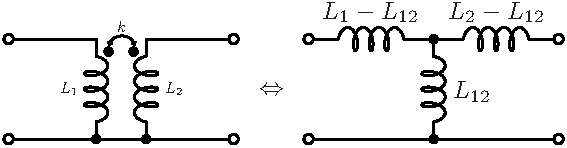
\includegraphics[scale=1]{fig/rasprezanje.pdf}
\caption{Уз распрезање калемова.}
\label{raspreg}
\end{figure}

\subsection{Савршени трансформатор}
Уколико је магнетска спрега трансформатора савршена, односно 
уколико нема магнетског расипања, $k = 1$, односно $L_{\rm 12} = \pm \sqrt{L_1 L_2}$,
такав трансформатор се назива \textbf{савршеним}. 
Без умањења  
општости, претпоставимо да су референтни смерови напона намотаја
одабрани тако да је $L_{\rm 12} = \sqrt{L_1 L_2}$. Тада се 
елиминацијом струја из модела спрегнутих калемова може показати да 
важи $\dfrac{v_1}{v_2 } = \sqrt[]{\dfrac{L_1}{L_2}}$. Пошто је 
сопствена индуктивност намотаја сразмерна квадрату броја навојака 
$L_i \propto N_i^2$, онда је и 
\begin{equation}
\boxed{
\dfrac{v_1}{N_1} = \dfrac{v_2}{N_2}
}
\end{equation}


\subsection{Идеални трансформатор}
Уколико посматрамо савршени трансформатор и за контуру средње 
линије језгра напишемо Уопштени Амперов закон имамо једначину 

\begin{equation}
N_1 i_1 + N_2 i_2 = \dfrac{B l}{\upmu_0 \upmu_r},
\label{uaz}
\end{equation}
где су 
$B$ интензитет вектора магнетске индукције у језгру, $l$ 
дужина средње линије језгра и $\upmu_{\rm r}$  релативна пермеабилност
материјала од кога је израђено језгро. Представимо број навојака оба намотаја нормализовано као $N_{i} = n_i N_0$ и заменимо у 
израз \eqref{uaz}. Тада $n_{i}$ представља релативни број 
навојака у односу на нормализациони фактор
$N_0$. За $N_0$ се може
одабрати, на пример, ред величине броја навојака оба намотаја. Уколико
су $N_1 = 1000$ и $N_2 = 2000$ онда се може одабрати на пример 
$n_1 = 1$ и $n_2 = 2$ за $N_0 = 1000$. Другим речима, са $n_i$ кодификујемо релативан број навојака намотаја а са $N_0$ њихов ред величине. Са тиме у виду 
једначину \eqref{uaz} можемо записати и као:
\begin{equation}
n_1 i_1 + n_2 i_2 = \dfrac{Bl}{\upmu_0 N_0 \upmu_r}
\end{equation}
Сада, приметимо да уколико је $\upmu_{\rm r}N_0 \to \infty$ онда 
једначина постаје $\boxed{n_1 i_1 + n_2 i_2 = 0}$. 
Тиме се добија модел \textbf{идеалног} 
трансформатора описан са две \textbf{алгебарске} једначине:

\begin{center}
\shadowbox{
\begin{minipage}{0.3\textwidth}
\textbf{\myul{Идеални трансформатор}}
\vspace*{0.5em}
\begin{itemize}
\item $
\dfrac{v_1}{n_1} = \dfrac{v_2}{n_2}
$
\item $i_1 n_1 + i_2 n_2 = 0$ 
\end{itemize}
\end{minipage}
%
\begin{minipage}{0.2\textwidth}
\begin{flushright}
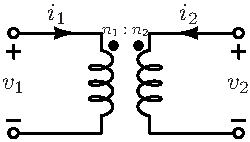
\includegraphics[scale=0.8]{fig/it-trafo.pdf}
\end{flushright}
\end{minipage}
}
\end{center}

\noindent
\begin{crtice}
Иако се 
материјал језгра при пројектовању 
може одабрати тако да $\upmu_{\rm r}$ буде велико, 
на пример трафо-лимови ($\upmu_{\rm r} \sim 100$), доступни материјали
постављају неку горњу границу пермеабилности. Са друге стране, инжењерским 
одабиром при пројектовању трансформатора може се одабрати велики 
број навојака намотаја тако да овај услов буде што боље задовољен.
На пример, уколико се пројектује трансформатор који треба да 
удвостручава напон, одабир $(N_1, N_2) = (200, 100)$ је бољи 
од одабира $(N_1, N_2) = (20, 10)$. To je углавном разлог 
зашто су скоро сви практични трансформатори са веома великим 
бројем намотаја, јер је често циљ направити што \textit{идеалнији}
трансформатор. 
Ипак, постоје и неки нарочити изузеци, као на пример Теслин 
трансформатор. 
За тачно одређивање потребног 
броја навојака постоје и други критеријуми, али ћемо се 
зауставити на овој илустрацији.
\end{crtice}

\subsection{Магнетизациона индуктивност}

Савршен трансформатор може се представити и помоћу 
идеалног трансформатора и једне индуктивности. Положај 
те индуктивности се 
може одабрати тако да се решавање кола 
највише поједностави
(са примарне или секундарне стране). Без доказа наводимо 
трансфигурацију: \\[0.5mm]
 

\shadowbox{
\begin{minipage}{0.3\textwidth}
\textbf{\myul{Магнетизациона индуктивност}}
\\[0.5mm]
 
$L_{\rm m} = L_1$ \\[0.5mm]

$n = \sqrt{\dfrac{L_2}{L_1}}$

\end{minipage}
%
\begin{minipage}{0.6\textwidth}
\begin{flushright}
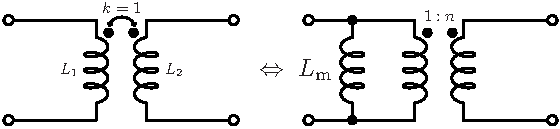
\includegraphics[scale=1]{fig/magnetizac.pdf}
\end{flushright}
\end{minipage}
}
